\documentclass[letterpaper, 12pt]{article}
\usepackage[letterpaper, top=2.5cm, bottom=2.5cm, left=3cm, right=3cm]{geometry} %margenes
\usepackage{fancyhdr} %formato de los encabezados de página
%personalización de los encabezados de página
\pagestyle{fancy} %estilo
\fancyhf{}
\fancyhead[L]{\textbf{Documentación}} %encabezado Esquina Superior Izquierda
\fancyhead[R]{\textbf{Proyecto de simulación}} %encabezado Esquina Superior Derecha
\fancyfoot[R]{\thepage}
\usepackage[utf8]{inputenc} %manejo de caracteres especiales
\usepackage[spanish]{babel} %manejo de encabezados de inglés a español
\usepackage{ragged2e} %alineado real justficado
\usepackage{graphicx} %manejo de imagenes
\usepackage{amsmath} %manejo de notación matemática
\usepackage{mathtools} %manejo de notación matemática
\usepackage{blindtext} %texto de relleno
\usepackage{amssymb} %manejo de simbología
\usepackage{float} %centrado de imagenes
\usepackage{hyperref} %manejo de enlaces e hipervínculos 
\usepackage{xcolor} %colores para enlaces hyperref
\usepackage[backend=biber]{biblatex}\addbibresource{bible.bib}

\hypersetup{ %colores de enlaces
    colorlinks = true,
    linkbordercolor = white, %sin borde
    linkcolor=black, %ENLACE NEGRO
    urlcolor=blue %URL AZUL
}

\nocite{*} %cita la bibliografia sin citar pedazos especificos en el texto

\begin{document}
    
    %PORTADA
    \begin{titlepage}
        \begin{figure}[ht]
            \centering
            
\includegraphics[width=15cm]{logosITT.png}
        \end{figure}
        \centering
        {\scshape\LARGE Tecnológico Nacional de México\\Instituto Tecnológico de Tijuana\par}
        \vspace{1cm}
        {\scshape\Large Simulación\par}
        \vspace{1cm}
        {\scshape\Large Proyecto de Simulación\par}
        \vspace{1.5cm}
        {\huge\bfseries Documentación: Simulación de una inversión en los \emph{meme stocks} en la bolsa de valores\par}
        \vspace{2cm}
        {\Large\itshape C. Abraham Jhared Flores Azcona\\19211640\par}
        \vfill
        Profesor: Ing. Diego Saul Vasquez Rios\par
    
        \vfill

        {\large 24 de junio de 2021}
    \end{titlepage}

    %indice
    \newpage
    \thispagestyle{empty}
    \tableofcontents
    \listoffigures

    %cuerpo
    \newpage
    \begin{justify}
        \setcounter{page}{1}
        \section{Introducción}
        \justify
        En esta documentación se muestran las tecnicalidades de la simulación de una inversión en \emph{meme stocks} como una tésis viable de inversión.
        \\\newline
        A lo largo de estos tiempos de pandemia, uno de los rubors que ha causado mayor furor en la web ha sido el de los ``inversionistas'' de \emph{wallstreetbets}
        que han cambiado el rubro conservador de las inversiones a un toque menos formas y más riesgoso. Esto se ha demostrado con el hito principal con las acciones de Gamestop
        que dejaron un gran precedente en la historia financiera global.
        \\\newline
        La finalidad de la documentación de este proyecto de simulación es mostrar las capacidades de cómputo de Microsoft Excel como una herramienta indispensable en el análisis de riesgo
        en los \emph{meme stocks} que han dejado marca en el mundo de las finanzas y tener un vestigio más formalizado de estas tésis del foro de \emph{wallstreetbets}.
        \section{Conceptos clave}
        \justify
        Se describe brevemente aquellas palabras que se usarán a lo largo de este escrito. Los conceptos son enfocados en finanzas, por lo que una buena base de las disciplinas financieras
        facilita la comprensión del texto restante.
        \begin{itemize}
            \item \textbf{Acciones:} el instrumento de inversión elegido. Para simpleza, se eligen cinco acciones.
            \item \textbf{Capital:} para los propositos de la redacción, es el dinero el cual se dispone para invertir.
            \item \textbf{Ganancia:} es la cantidad de dinero que se gana dada la inversión. Generalmente se expresa como porcentaje.
            \item \textbf{MXN:} es la abreviación técnica del peso mexicano.
            \item \textbf{Paridad peso-dolar:} se refiere a la tasa de cambio de un peso mexicano covertido a un dólar estadounidense.
            \item \textbf{Tasa de inflación:} el porcentaje por el cual la cantidad de capital pierde poder adquisitivo (su valor baja a travéz del tiempo).
            \item \textbf{Ticker:} es la abreviación de la acción en la bolsa de valores de la compañia deseada.
            \item \textbf{USD:} abreviación técnica del dólar estadounidense.
            \item \textbf{Volatilidad:} el porcentaje del cambio de precio de una acción. Se interpreta que mientras más alto sea el porcentaje, el cambio es más drástico.
        \end{itemize}
        \section{Antecedentes}
        \justify
        El sub-reddit de \emph{wallstreetbets} se ha convertido en uno de los foros más populares de reddit por sus tendencias de ``inversión'' con instrumentos sumamente riesgosos por lo que muchos de
        sus éxitos o fracasos se consideran apuestas, que es parte del nombre del foro. Uno de los hitos recientes de \emph{wallstreetbets} ha sido con las acciones de la compañia Gamestop.
        \\\newline
        El realizar una simulación con el enfoque a la bolsa de valores tampoco es algo nuevo. Distintos videos en Youtube explican con detalle y simpleza las distintas maneras sobre el como plantear un proyecto de Excel
        que funcione con el objetivo de simular los rendimientos de la bolsa de valores.
        \section{Planteamiento}
        \justify
        Se desarrolló una simulación de inversión en cinco acciones que son populares en \emph{wallstreetbets} para observar si los rendimientos en las acciones
        populares son realmente una buena tésis de inversión y por ende, una buena opción como una inversión seria. Dichas accionas se llaman coloquialmente como \emph{meme stocks} ya que dichas acciones
        se convierten en meme y ganan popularidad como instrumentos de inversión dentro del foro.
        \section{Hipótesis}
        \justify
        La primer hipótesis es que teniendo el consenso del foro, se puede mediar la posibilidad del éxito ó fracaso de la inversión.
        \\\newline
        La segunda hipótesis es que mientras mas volatididad tenga una acción, se puede tener más riesgo y mayor ganancia. 
        \\\newline
        La tercera hipótesis recae en si se debe mantener la inversión por lo menos por un año para obtener mayores ganancias sobre el capital invertido.
        \\\newline
        La cuarta y última hipótesis es si mientras más capital invertido máyor la posibilidad de pérdida ó de ganancia.        
        \section{Objetivos}
        \justify
        El primer objetivo es probar si una tésis de inversión en base al consenso y popularidad de ciertas acciones dentro de un foro de discusión es viable para poder ser aplicada como una estrategia de inversión.
        \\\newline
        El segundo objetivo es observar el comportamiento de las acciones y su volatilidad para mediar el rendimiento futuro de la inversión dado el capital invertido y sus posibles ganancias.
        \\\newline
        El tercer objetivo es observar los posibles rendimentos y definir si es conveniente administrar de manera frecuente las posiciones.
        \\\newline
        El cuarto objetivo es determinar si los rendimientos de la inversión en las acciones específicadas supera los rendimientos del índice de mercado S\&P 500.
        \\\newline
        Finalmente, el quinto objetivo es apreciar la ayuda del cómputo como una herramienta útil en la toma de desiciones de carácter financiero.
        \section{Justificación}
        \justify
        El realizar simulaciones con el aspecto financiero en mente permite probar (hasta cierto punto) si nuestro prospecto de inversión es viable permitiendo el seguir desarrollando
        la idea de inversión o descartar dicha idea para formular otra ya que en procesos estocásticos tan remarcables como la valuación del precio de una acción en la bolsa de valores
        es imposible ``atinarle al precio''.
        \\\newline
        Lo anterior es relevante ya que a lo largo del tiempo, cambios drásticos al precio de una acción pueden beneficiar o maleficiar el prospecto de ganancias, y por ende, afectar el plazo deseado de inversión
        para tener mayores ganancias, o mediar pérdidas no realizadas, a pesar de que el mercado recae en cierto grado en las interacciones de los actores que participan en la bolsa, que es un corolario del sentimiento del mercado.
        \\\newline
        También es de suma importancia el realizar simulaciones de este ámbito para proyectar si se debe estar revisando de manera rutinaria las acciones elegidas para ``atinarle al precio'' o si es más viable y cómodo esperar al plazo dado,
        que para la simulación de inversión, es de un año bursátil. Se debe tener en cuenta que el revisar de manera constante una posición puede residuar en impulsos emocionales que afecten a la inversión y a la sanidad mental del inversionista.
        \\\newline
        Finalmente, comparar nuestros rendimientos con uno de los índices más populares (y uno de los más viejos) nos indica si es más congruente ingresar el capital a invertir en el S\&P 500 en el mismo plazo o seguir con la tésis de las cinco acciones
        bursatiles elegidas.
        \section{Marco teórico}
        \justify
        Esta simulación está aplicando la tesis de valuación por medio de la Teoría de la Caminata Aleatoria.
        Esta Teoría de la Caminata Aleatoria es un modelo matemático de la bolsa de valores. Los proponentes de la teoría
        creen que los precios de las acciones dentro del mercado evolucionan acorde a una caminata aleatoria.
        \\\newline
        La implicación relevante a esta simulación es que para los inversionistas es imposible sobrepasar el promedio del rendimiento del mercado
        mas allá que por mera suerte, que para los términos prácticos de la simulación se traduce a que se tiene una media de 0 para los rendimientos. 
        Los preponentes de esta estratégia recomiendan usar la estrategia de ``comprar y mantener'' con un fondo indizado, tal como el S\&P 500.
        \\\newline
        También es relevante tener en cuenta la noción de la distribución normal. Esto es debido a que en las inversiones se tienen dos aspectos generalmente
        universales: riesgo y ganancia. Dicha distribución normal cuantifica ambos aspectos por la media de ganancia y la volatidad para el riesgo ya que los cambios
        en las razones de cambio de precio se asumen que están normalmente distribuidas.
        \section{Definición de la población y muestra}
        \justify
        Para los términos financieros de esta simulación, se van a emplear los rendimientos anuales de 5 acciones de la bolsa americana de valores que fueron las cinco acciones más populares del foro hasta el 28 de abril del 2021, los cuales son:
        \begin{itemize}
            \item AMD \textbf{(\$AMD)}.
            \item Gamestop \textbf{(\$GME)}.
            \item MicroVision \textbf{(\$MVIS)}.
            \item Palantir Technologies \textbf{(\$PLTR)}.
            \item Tesla Motors \textbf{(\$TSLA)}.
        \end{itemize}
        \section{Formulación del sistema y del modelo}
        \justify
        A continuación se muestra el modelo del sistema para la simulación:
        \begin{figure}[H]
            \centering
            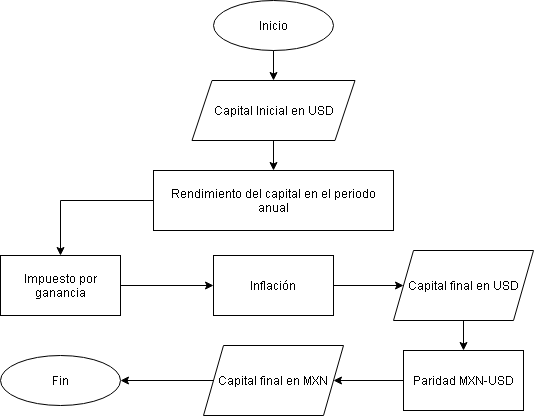
\includegraphics[width=14cm,height=6cm]{FlowchartSIMULATION.png}
            \caption{Diagrama de flujo del modelo del sistema a simular.}
        \end{figure}
        \justify
        Donde:
        \begin{itemize}
            \item \textbf{Capital inicial en USD:} el dinero a invertir en las cinco acciones susodichas.
            \item \textbf{Rendimiento del capital en el periodo anual:} que porcentaje de perdida o ganancia se tuvo en las cinco acciones.
            \item \textbf{Impuesto por ganancia:} el porcentaje que se debe de descontar a las ganancias despues del periodo para destinarlas a las contribuciones tributarias de la legislación aplicable.
            \item \textbf{Inflación:} porcentaje de perdida del poder adquisitivo.
            \item \textbf{Capital final en USD:} el dinero obtenido en dolares estadounidenses después del periodo y prospecto de inversión.
            \item \textbf{Paridad MXN en USD:} el cambio de moneda de dolares estadounidenses a pesos mexicanos.
            \item \textbf{Capital final en MXN:} el dinero obtenido en pesos mexicanos.
        \end{itemize}
        \section{Recolección de datos}
        \justify
        Se recolectaron los rendimientos a un año de inversión por medio de consultas breves de dichos rendimientos en la página web de Yahoo Finance, que posteriormente se descargó como tablas de Excel para alimentar a la simulación.
        \section{Implementación del modelo en la computadora}
        \justify
        La herramienta computacional para implementar el modelo es Microsoft Excel ya que ha sido la principal herramienta en la que nos hemos familiarizado para resolver estas tareas que no requieren tanta complejidad computacional.
        \\\newline
        Aparte, las simulaciones de Monte Carlo que se realizaron a lo largo del semestre nos permite tener platillas a usar, facilitando el desarrollo de la simulación deseada sin tantos preámbulos.
        \\\newline
        En lo que respecta del formato, se decidió utilizar alrededor de 6 hojas dentro de la hoja de cálculo que corresponden al siguiente listado:
        \begin{itemize}
            \item \emph{\textbf{Overview:}} Datos generales para la simulación y sus resultados relevantes.
            \item \emph{\textbf{\$AMD:}} Muestra los datos principales para la simulación del rendimiento, incluyendo cambios de precio y la volatididad.
            \item \emph{\textbf{\$GME:}} \dots
            \item \emph{\textbf{\$MVIS:}} \dots
            \item \emph{\textbf{\$PLTR:}} \dots
            \item \emph{\textbf{\$TSLA:}} \dots
        \end{itemize}
        \subsection{\emph{Overview}}
        \justify
        Para esta hoja el formato quedó de la siguiente manera:
        \begin{figure}[H]
            \centering
            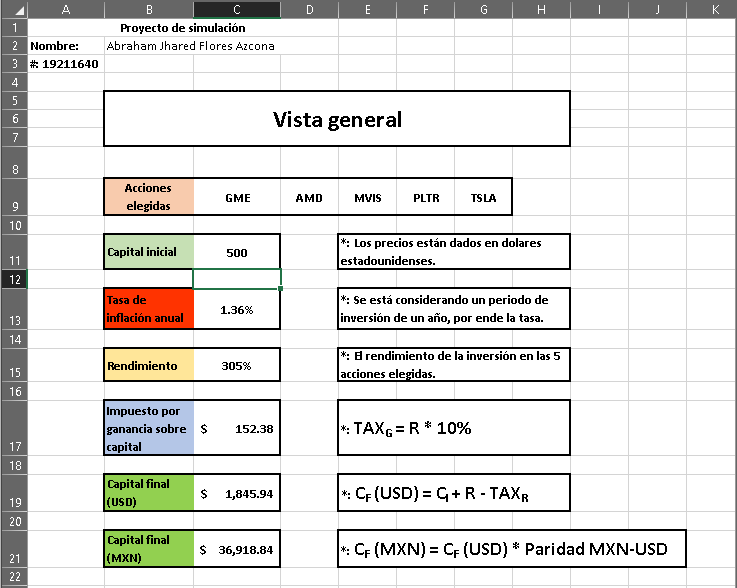
\includegraphics[height=8cm,width=14cm]{formato_overview.PNG}
            \caption{Formato de la hoja \emph{Overview} del documento de simulación en Excel.}
        \end{figure}
        \justify
        A grandes rasgos, se tienen las acciones elegidas para realizar el proceso de simulación como el primer registro de la hoja. 
        El capital inicial dado en USD como el segundo registro en color verde claro. En el tercer registro remarcado con color rojo se tiene la tasa de inflación anual
        que decrementa el valor de nuestros rendimientos como una constante. El rendimiento encontrado en color amarillo como el cuarto registro de la hoja expresa el porcentaje de ganancia o pérdida general de la inversión. En el quinto registro de color azul tenemos el impuesto por ganancia
        sobre capital el cual es aplicado con el supuesto de que el inversionista es ciudadano mexicano, por lo que en base a la legislación fiscal vigente a la fecha de entrega de la documentación es de un 10\% sobre dicha ganancia. Finalmente en el sexto y séptimo registro de color verde se 
        tiene el capital final en USD y MXN respectivamente.
        \\\newline
        Las formulas de Excel empleadas en la hoja son las siguientes: 
            \begin{verbatim}
Rendimiento = '$AMD'!<Rendimiento>+'$GME'!<Rendimiento>+
'$TSLA'!<Rendimiento>+'$PLTR'!<Rendimiento>+'$MVIS'!<Rendimiento>

Impuesto por ganancia: =(<Capital_inicial>*<Rendimiento>)*10%

Capital final (USD): =((<Capital_inicial>+<Capital_inicial>*
<Rendimiento>))-((<Capital_inicial>*<Rendimiento>)-
<Impuesto_por_ganancia>)*C13

Capital final (MXN): =<Capital_inical_USD>*<Paridad_MXN-USD>\end{verbatim}
        \subsection{\emph{\$AMD, \$GME, \$MVIS, \$PLTR y \$TSLA}}
        \justify
        El formato general para las acciones es el siguiente:
        \begin{figure}[H]
            \centering
            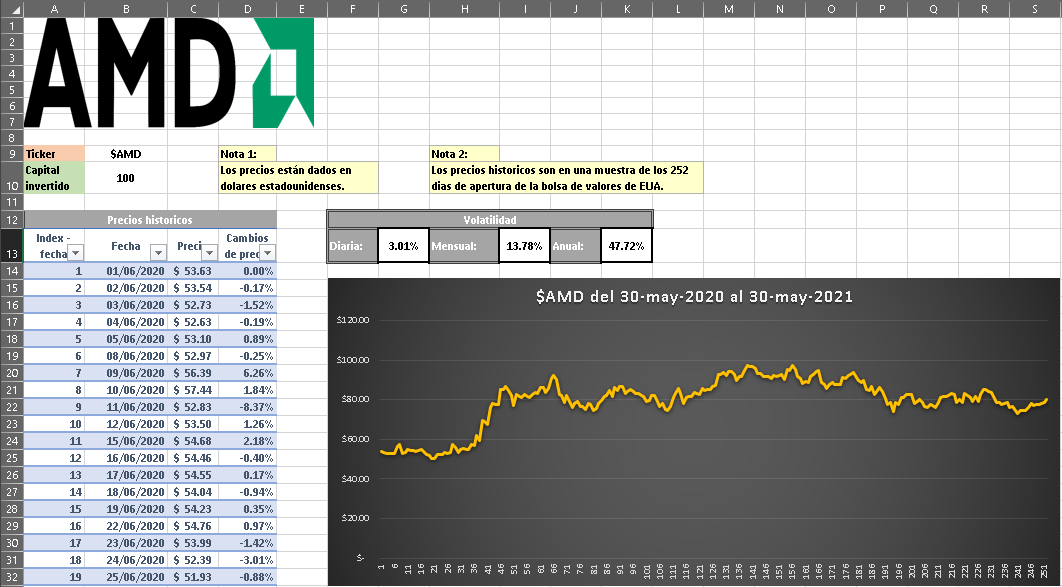
\includegraphics[height=12cm,width=14cm]{formato_acciones_1.PNG}
            \caption{Formato de la primer parte de la hoja \emph{\$AMD} del documento de simulación en Excel.}
        \end{figure}
        \justify
        Tomando como referencia el formato de esta primer parte para las demás hojas, tenemos la imágen del logotipo de la compañia de dicha acción, el ticker, la cantidad de capital invertido para dicha acción, notas aclaratorias para las magnitudes de las cantidades y demás, los precios historicos
        diarios por un año bursátil con los cambios de precio, las volatilidades diarias, mensuales y anuales y una gráfica del movimiento de la acción al periodo de un año bursatil con los precios historicos.
        \begin{figure}[H]
            \centering
            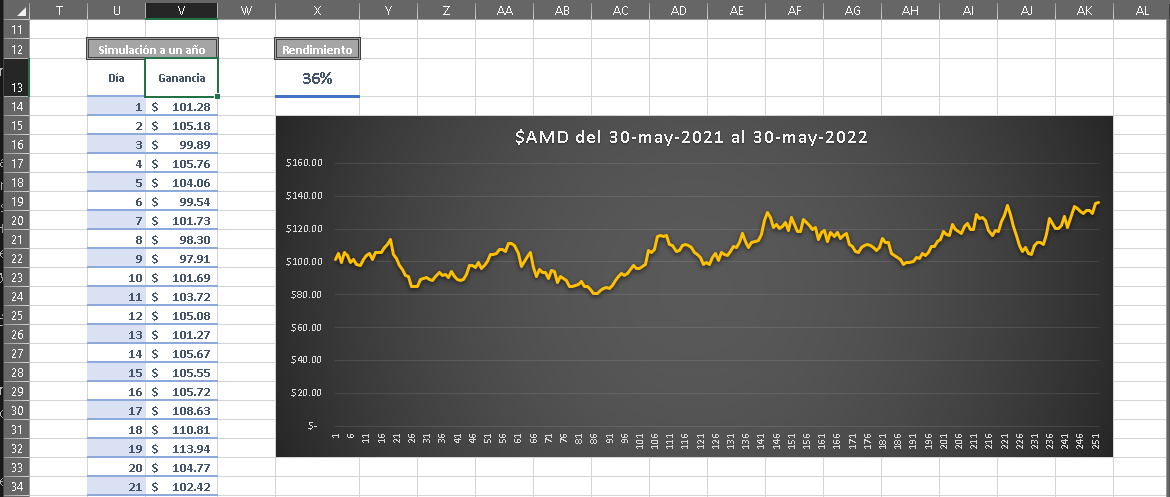
\includegraphics[height=8cm,width=14cm]{formato_acciones_2.PNG}
            \caption{Formato de la segunda parte de la hoja \emph{\$AMD} del documento de simulación en Excel.}
        \end{figure}
        \justify
        En lo que respecta de la segunda parte, tenemos los días y la ganancia en la tabla de ``Simulación a un año'', la columna que contiene el porcentaje de rendimiento de la inversión a un año bursatil con la simulación empleada.
        \\\newline
        Las formulas de Excel empleadas en la hoja son las siguientes: 
            \begin{verbatim}
Capital invertido: =Overview!C11/5

Cambios de precio (1er. día): 0

Cambios de precio (resto de los dias): =LN(<actual>/<anterior>)

Volatilidad diaria: =STDEV.P(Precios_AMD[Cambios de precio])

Volatilidad mensual: =<volatilidad_diaria>*SQRT(21)

Volatilidad anual: =<volatilidad_diaria>SQRT(252)

Ganancia de simulación a un año (1er. día): =<capital_invertido>*
(1+NORMINV(RAND(),0,<$volatilidad$diaria>))

Ganancia de simulación a un año (resto de los días): 
<ganancia_anterior>*(1+NORMINV(RAND(),0,<$volatilidad$diaria>))

Rendimiento: (<ganancia_simulación_(día_255)>-<capital_inicial>)/
<capital_inicial>\end{verbatim}
        \section{Análisis de resultados} %falta redactar
        \justify
        La ejecución de la simulación arrojó los siguientes resultados a 100 simulaciones elijiendo el rendimiento de la 
        hoja \emph{Overview} y comparando a estos con el rendimiento anual del S\&P 500 del año 2020 (15.8\%):
        \begin{itemize}
            \item \textbf{Cantidad de rendimientos que superaron el rendimiento anual del S\&P 500:} 21.
            \item \textbf{\dots que no superaron \dots:} 79.
            \item \textbf{Media de rendimientos \(\left(\overline{X}\right)\):} 54\%.
            \item \textbf{Moda de rendimientos \(\left(\hat{X}\right)\):} .
            \item \textbf{Rendimiento mayor \(\left(\text{Max}\left(X\right))\right)\):} 12144\%.
            \item \textbf{\dots menor \(\left(\text{Min}\left(X\right)\right)\):} -388\%.
            \item \textbf{Volatilidad \((\sigma)\):} 1291\%.
        \end{itemize}
        Esto confirma la principal sospeccha de que la volatilidad de las acciones recae en prospectos muy maleficiosos para la inversión. Solo el 21\%
        intentos de inversión superaron el rendimento anual del S\%P 500 y de estas, solo una aumentó diez veces el capital invertido.
        \\\newline
        Debido a que los porcentajes de rendimiento son multiplicaciones al capital, se infiere que mientras más grande sea el capital, más grande el prospecto de pérdida y de ganancia.
        \\\newline
        Finalmente, el consenso popular alrededor de estas acciones no indica de manera certera la posibilidad de éxito en la inversión. 
        \section{Conclusiones y recomendaciones}
        \justify
        El usar las herramientas de cómputo a nuestra dispocisión auxilia en altos grados de magnitud nuestros prospectos
        en las acciones que se desee invertir. No necesariamente equivale a que tengamos un buen prospecto, lo cual es congruente
        en un sistema excesivamente complejo como la bolsa de valores, donde una teoría matemática no equivale a que sea la ``mina de oro'' 
        de la modelación financiera teniendo en cuenta que influyen aspectos sociales, psicológicos, legislativos, etc.
        \\\newline
        Claro está que si se desea invertir en acciones que son populares en foros, habrá un mayor riesgo ya que no necesariamente existe un
        sustento para estas elecciones, por lo que se recomienda que se proceda con precaución al momento de elegir que acciones invertir si son basadas
        en consensos como estos. Es más rentable invertir en un fondo indizado si realmente se desea invertir sin tantas preocupaciones por volatilidad.
    \end{justify}

    %bibliografía
    \newpage
    \renewcommand{\headrulewidth}{0pt}
    \renewcommand{\footrulewidth}{0pt}
    \fancyhead[L]{}
    \fancyhead[R]{}
    \fancyfoot[R]{\thepage}
    \printbibliography[heading=bibintoc]

\end{document}